\chapter{Dataset}

\section{Study Area}
The study area, with an area of 100 $km^2$, is located in southeastern France, centered on the city of Balaruc-les-Bains, bordering the Mediterranean Sea. 
It is a small and densely populated urban area surrounded by agricultural crops, mainly vineyards, and natural vegetation.
Figure \ref{fig:gtmap} shows the GT map overlaid on the Sentinel-2 image taken on January 2019.

\begin{figure}[H]
  \centering
  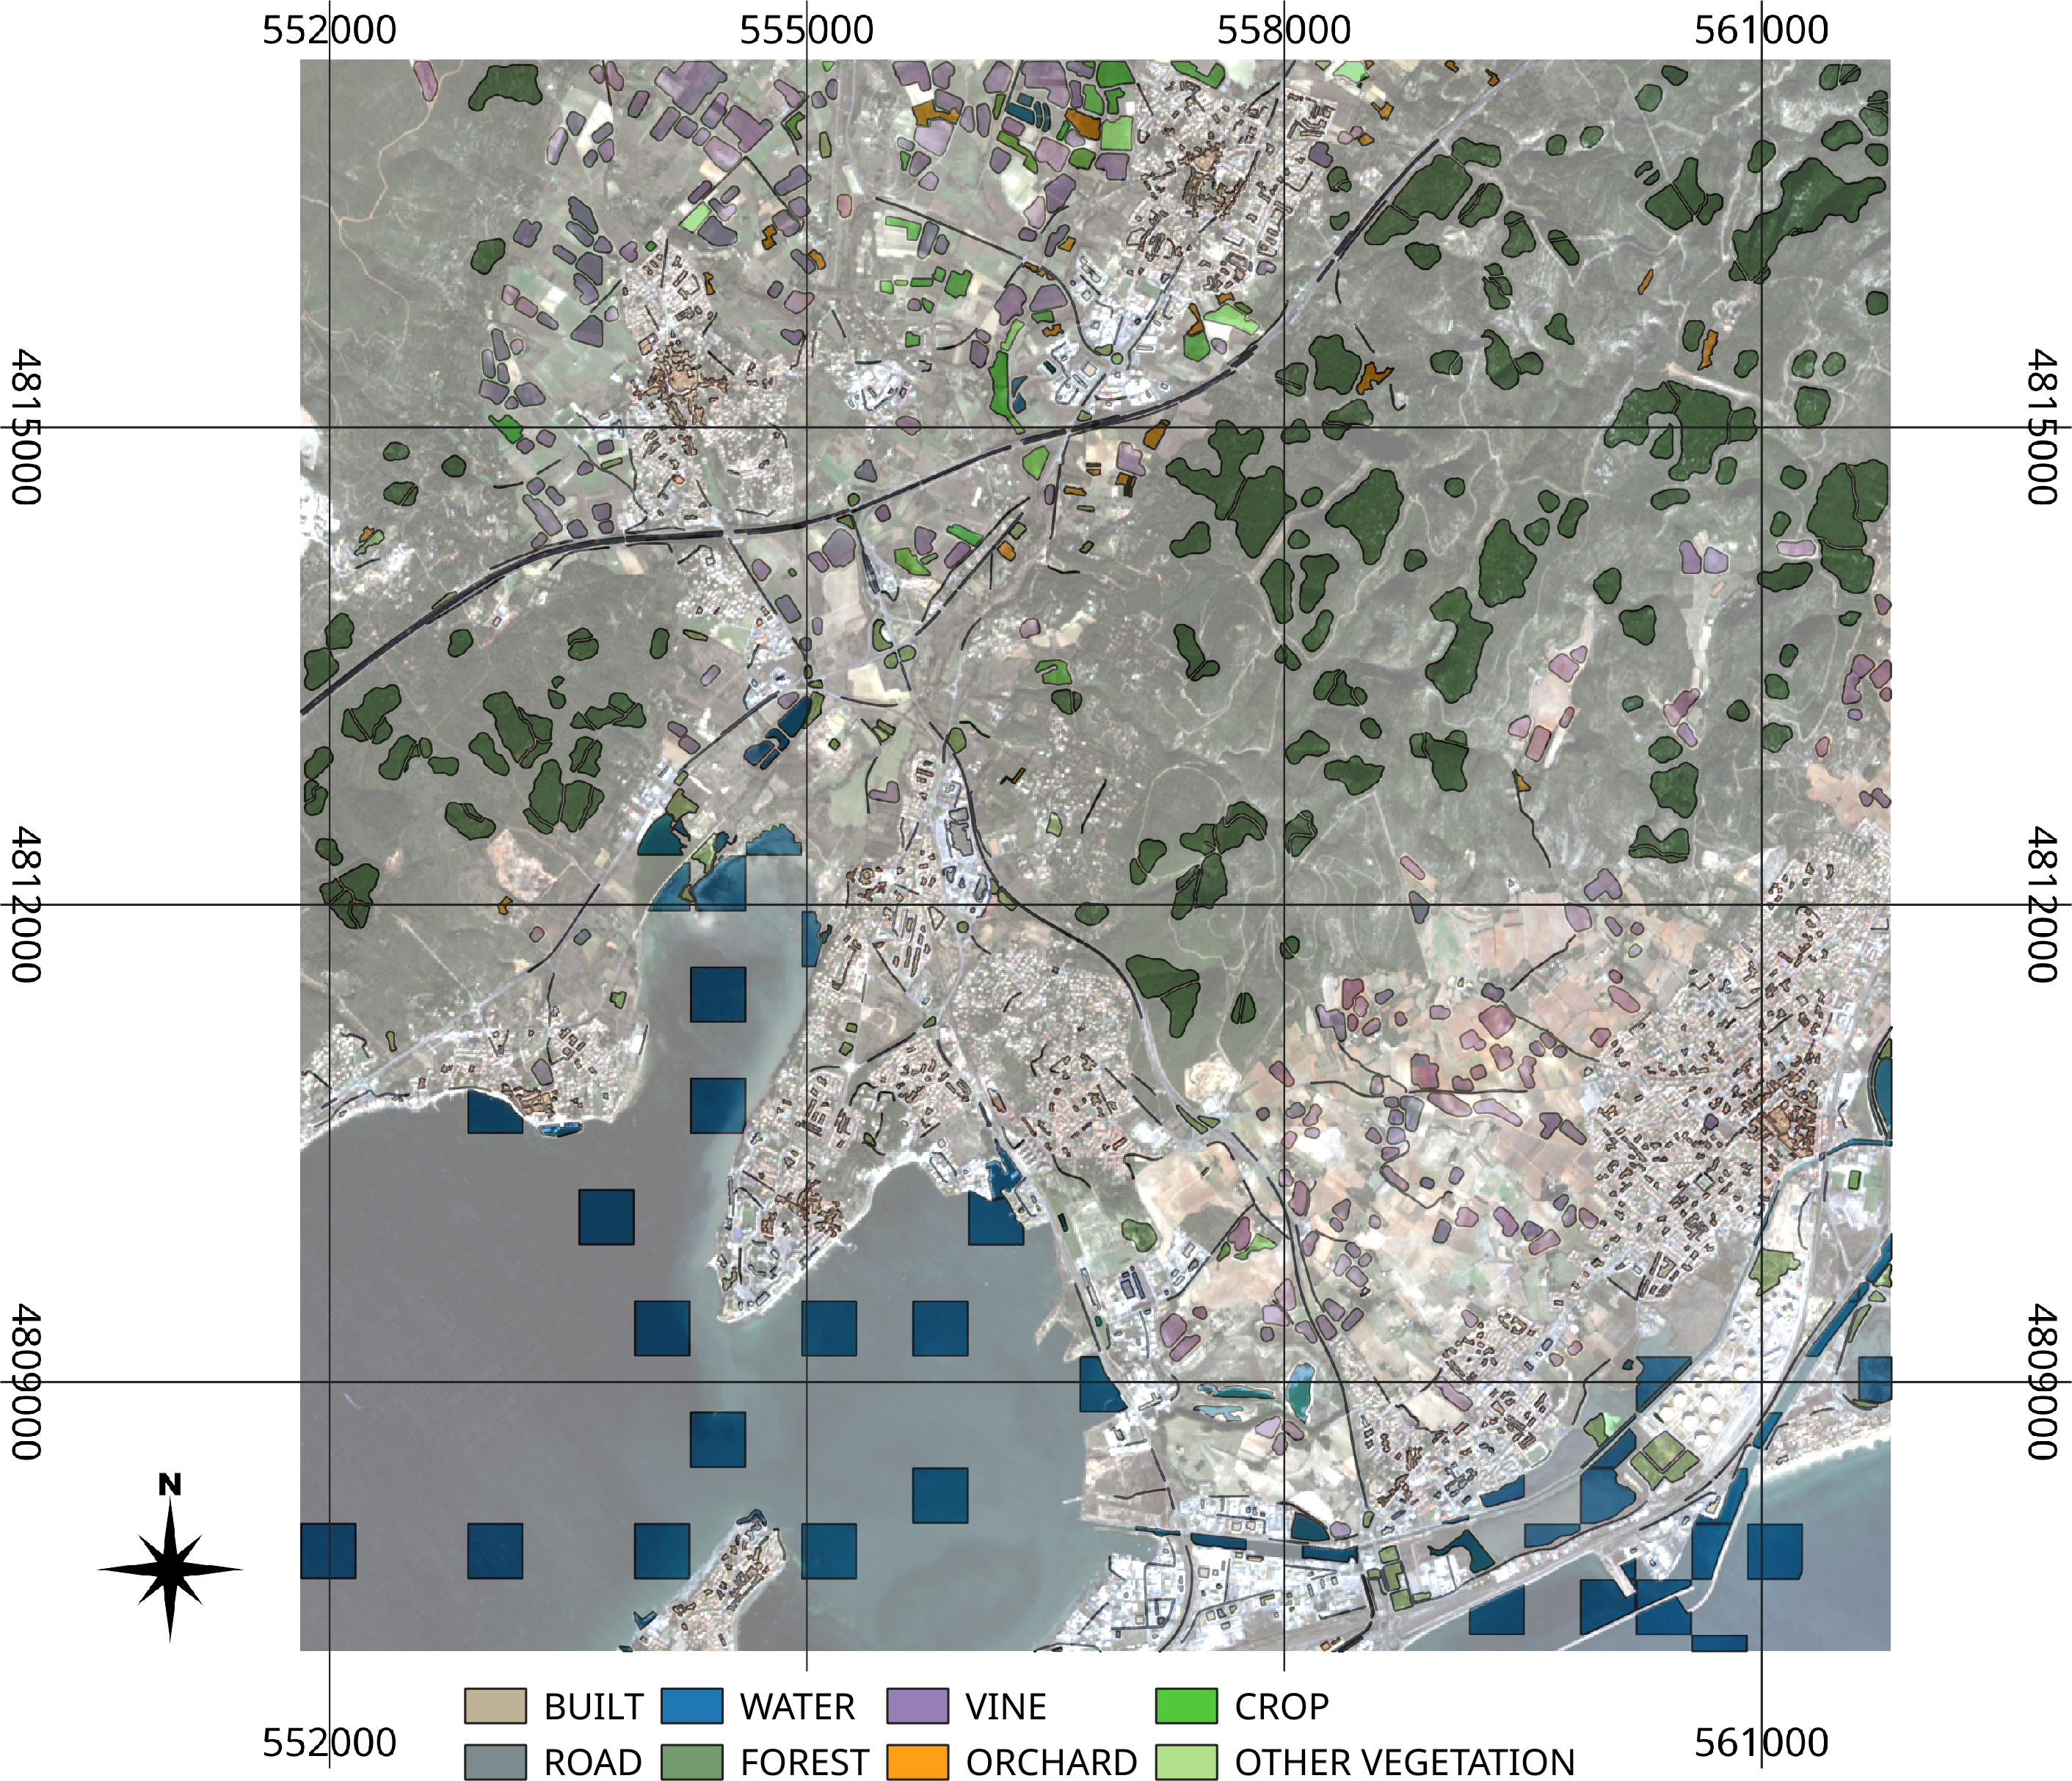
\includegraphics[width=1\textwidth]{BLC_20180123_SAT-GT_300dpi.png}
  \caption{The Sentinel-2 image is overlaid with ground truth data.}
  \label{fig:gtmap}
\end{figure}


\section{Chronology}

\textit{Satellite Image Time Series:} 
% TODO: rephrase this
A total of 54 Sentinel-2 image time series covering the year 2019 were collected for the study. 
The images were selected to represent the temporal (annual) evolution of the land cover associated with the study area and to filter out images that were heavily affected by cloud phenomena.
The acquisition dates of the Sentinel-2 satellite image time series are shown in Figure \ref{fig:sitsdates}.

\begin{figure}[H]
  \centering
  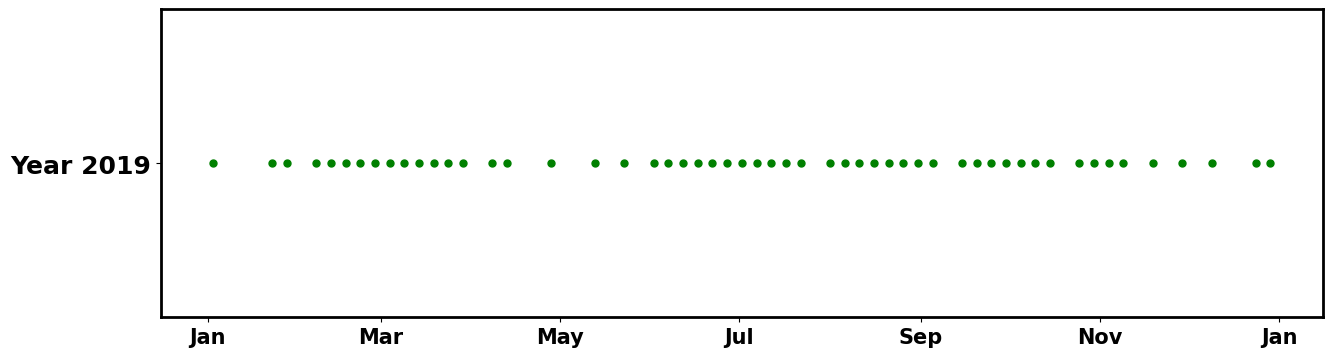
\includegraphics[width=1\textwidth]{SITSdates}
  \caption{Acquisition dates of each Satellite Image Time Series.}
  \label{fig:sitsdates}
\end{figure}

\section{Mask and Bands}


The images used in this analysis were obtained from the THEIA pole platform\footnote{\url{http://theia.cnes.fr}} at level-2A in top of canopy reflectance values and with associated cloud masks.

% TODO: ask dino about the bands
% TODO: tell what the 16 bands are
We considered only the 10-m spatial resolution bands, namely blue, green, red, and near-infrared.

To replace cloudy pixel values, a preprocessing step was performed using multi-temporal linear interpolation based on the available cloud masks (also known as temporal gap-filling\cite{IENCO201911}).
The study area is located within the Sentinel-2 tile 31TEJ with relative orbit number 8.

The missing ratio in the dataset used for this study is 33.9\%. It is important to note that this missing ratio refers specifically to cloud masks.

\section{Ground Truth Data}

The ground truth data was built from various sources: the \textit{Registre Parcellaire Graphique} (RPG) reference data (the French land parcel identification system), the French National Geographic Institute \textit{‘BD-Topo \& BD Forêt’} and the visual interpretation of a SPOT 6 image (to assess and enrich the GT data) as well. 
The GT was assembled in Geographic Information System (GIS) vector file, containing a collection of polygons, each attributed with a land cover category. 
Statistics about the GT data are reported in Table \ref{tab:gt}.

\begin{table}[H]
\centering
\begin{tabular}{lcrr}
  Class Name & Class ID. & \# Polygons & \# Pixels \\[0.2cm]\hline \\[-0.2cm] 
  Built & 1 & 712 & 10,412\\
  Road  & 2 & 328 & 5,165\\
  Water & 3 & 82 & 32,095\\
  Forest  & 4 & 172 & 49,175\\
  Vine  & 5 & 223 & 28,667\\
  Orchard & 6 & 32 & 2,075\\
  Crop  & 7 & 39 & 5,205\\
  Other Vegetation & 8  & 56 & 4,812 \\[0.2cm]\hline \\[-0.2cm] 
  & Total & 1,644 & 137,606
\end{tabular}
\caption{Number of polygons and pixels for each class.}
\label{tab:gt}
\end{table}


